\subsection{第一存在定理}

定义 1. 设 A、A' 是两个环，h: A → A' 是环同态。若 \iffalse h\^{}\{-1\}(a')\fi\(a = h^{-1}(a')\)，则称 A' 的理想 a' 位于 A 的理想 a 之上。

因此，说素理想 \(\mathfrak{p}'\) （\(\mathbf{A}'\) 的）位于理想 \(\mathfrak{p}\) （\(\mathbf{A}\) 的）之上，就是指 \(\mathfrak{p}\) 是 \(\mathfrak{p}'\) 在连续映射 \(^a h\) ： \(\operatorname{Spec}(\mathbf{A}') \to \operatorname{Spec}(\mathbf{A})\) （它与 \(h\) 相伴）下的像（第 II 章，§ 4，第 3 节）。

注意，为使 \(\mathbf{A}'\) 中存在位于 \(\mathbf{A}\) 的理想 (0) 之上的理想，必须而且只需 \(h: \mathbf{A} \to \mathbf{A}'\) 是单射。

设 \(\mathfrak{a}\) 是 \(\mathbf{A}\) 的理想；对 \(h\) 取商，得到同态 \(h_1: \mathbf{A} / \mathfrak{a} \to \mathbf{A}' / \mathfrak{a}'\) ；说 \(\mathfrak{a}'\) 是 \(\mathbf{A}'\) 的位于 \(\mathfrak{a}\) 之上的理想，等价于说 \(\mathfrak{a}\mathbf{A}' \subset \mathfrak{a}'\) 且 \(\mathfrak{a}' / \mathfrak{a}\mathbf{A}'\) 是 \(\mathbf{A}' / \mathfrak{a}\mathbf{A}'\) 的位于 (0) 之上的理想。

引理 1. 设 \(h: \mathbf{A} \to \mathbf{A}'\) 是环同态，\(\mathbf{S}\) 是 \(\mathbf{A}\) 的乘性子集，\(i = i_{\mathbf{A}}^{\mathbf{S}}: \mathbf{A} \to \mathbf{S}^{-1}\mathbf{A}\) ，\(i' = i_{\mathbf{A}'}^{h(\mathbf{S})}: \mathbf{A}' \to \mathbf{S}^{-1}\mathbf{A}' = (h(\mathbf{S}))^{-1}\mathbf{A}'\) 是典范同态，而 \(h_1 = \mathbf{S}^{-1}h: \mathbf{S}^{-1}\mathbf{A} \to \mathbf{S}^{-1}\mathbf{A}'\) ，于是有交换图

\pandocbounded{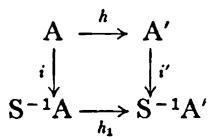
\includegraphics[keepaspectratio]{images/part002_a0a90333.jpg}}

设 \(\mathfrak{p}\) 是 \(\mathbf{A}\) 的素理想且 \(\mathfrak{p} \cap \mathbf{S} = \varnothing\) 。则 \(\mathfrak{a}' \mapsto \mathbf{S}^{-1}\mathfrak{a}'\) 是从集 \(\mathcal{F}\) ——\(\mathbf{A}'\) 的位于 \(\mathfrak{p}\) 之上的理想组成的集——到集 \(\mathcal{F}_1\) ——\(\mathbf{S}^{-1}\mathbf{A}'\) 的位于 \(\mathbf{S}^{-1}\mathfrak{p}\) 之上的理想组成的集——上的满射，而映射 \(\mathfrak{a}_1' \mapsto i'^{-1}(\mathfrak{a}_1')\) 是 \(\mathcal{F}_1\) 到 \(\mathcal{F}\) 中关于 \(h(S)\) 饱和的理想组成的集上的双射；特别地，\(\mathfrak{p}' \mapsto \mathbf{S}^{-1}\mathfrak{p}'\) 是从 \(\mathbf{A}'\) 的位于 \(\mathfrak{p}\) 之上的素理想组成的集到 \(\mathbf{S}^{-1}\mathbf{A}'\) 的位于 \(\mathbf{S}^{-1}\mathfrak{p}\) 之上的素理想组成的集上的双射。

我们知道 \(\mathbf{S}^{-1}\mathfrak{p}\) 是 \(\mathbf{S}^{-1}\mathbf{A}\) 的素理想，且 \(i^{-1}(\mathbf{S}^{-1}\mathfrak{p}) = \mathfrak{p}\) （第 II 章，§ 2，第 5 节，命题 11）；若存在理想 \(\mathfrak{b}'\) （\(\mathbf{S}^{-1}\mathbf{A}'\) 的位于 \(\mathbf{S}^{-1}\mathfrak{p}\) 之上的理想），则 \(h(i'^{-1}(\mathfrak{b}')) = i^{-1}(h_1(\mathfrak{b}')) = \mathfrak{p}\) ；由于 \(\mathbf{S}^{-1}.i'^{-1}(\mathfrak{b}') = \mathfrak{b}'\) （同前），这已经表明 \(\mathcal{F}\) 在映射 \(\mathfrak{a}'\mapsto\mathrm{S}^{-1}\mathfrak{a}'\) 下的像包含 \(\mathcal{F}_{1}\) 。另一方面，若 \(\mathfrak{a}'\in\mathcal{F}\) ，\(a\in\mathbf{A}\) 且 \(s\in\mathbf{S}\) ，则有下列等价关系

\[
\begin{array}{l} h _ {1} (a / s) \in \mathrm{S} ^ {- 1} \mathfrak {a} ^ {\prime} \Leftrightarrow h (a) / h (s) \in \mathrm{S} ^ {- 1} \mathfrak {a} ^ {\prime} \\ \Leftrightarrow \text { there   exists } t \in \mathrm{S} \text { such   that } h (t) h (a) \in \mathfrak {a} ^ {\prime} \\ \Leftrightarrow \text { there   exists } t \in \mathrm{S} \text { such   that } t a \in \mathfrak {p} \\ \Leftrightarrow a / s \in \mathrm{S} ^ {- 1} \mathfrak {p}. \end{array}
\]

于是 \(h_1^{-1}(\mathbf{S}^{-1}\mathfrak{a}') = \mathbf{S}^{-1}\mathfrak{p}\) ，这就完成了 \(\mathcal{F}\) 在映射 \(\mathfrak{a}' \mapsto \mathbf{S}^{-1}\mathfrak{a}'\) 下的像等于 \(\mathcal{F}_1\) 的证明；其余断言由第 II 章，§ 2，第 5 节，命题 11 得出。

命题 1. 设 \(h: \mathbf{A} \to \mathbf{A}'\) 是环同态且 \(\mathbf{A}'\) 在 \(\mathbf{A}\) 上是整的，\(\mathfrak{p}'\) 是 \(\mathbf{A}'\) 的素理想，而 \(\mathfrak{p} = h^{-1}(\mathfrak{p}')\) 。为使 \(\mathfrak{p}\) 极大，必须而且只需 \(\mathfrak{p}'\) 极大。

记 \(\mathrm{B} = \mathrm{A} / \mathfrak{p}\) ，\(\mathrm{B}' = \mathrm{A}' / \mathfrak{p}'\) ，并设 \(h_1 \colon \mathrm{B} \to \mathrm{B}'\) 是对 \(h\) 取商得到的同态；\(\mathrm{B}\) 与 \(\mathrm{B}'\) 是整环，且 \(\mathrm{B}'\) 在 \(\mathrm{B}\) 上是整的（§ 1，第 1 节，命题 2）。说 \(\mathfrak{p}\) （相应地 \(\mathfrak{p}'\) ）极大，就是指 \(\mathrm{B}\) （相应地 \(\mathrm{B}'\) ）是域。于是命题由下述引理得出：

引理 2. 设 B 是整环，A 是 B 的子环且 B 在 A 上是整的。为使 B 是域，必须而且只需 A 是域。

若 A 是域，则对 B 中所有 \(y \neq 0\) ，A[y] 按假设（ \(\S 1\) ，定理 1）是有限生成的 A-模；由于 A[y] 是整环，它是域（《代数》，第 V 章，\(\S 2\) ，第 1 节，命题 1），更不必说 y 在 B 中可逆，因而 B 是域。反之，设 B 是域，并设 A 中 \(z \neq 0\) ；由于 \(z^{-1} \in B\) ，\(z^{-1}\) 在 A 上是整的，换言之存在整依赖方程

\[
z ^ {- n} + a _ {1} z ^ {- (n - 1)} + \dots + a _ {n} = 0
\]

其中 \(a_{i} \in \mathbf{A}\) ；而这关系式表明

\[
- z ^ {- 1} = a _ {1} + a _ {2} z + \dots + a _ {n} z ^ {n - 1} \in A,
\]

因而 A 当然是域。

推论 1. 设 \(h: \mathbf{A} \to \mathbf{A}'\) 是环同态且 \(\mathbf{A}'\) 在 \(\mathbf{A}\) 上是整的，\(\mathfrak{p}\) 是 \(\mathbf{A}\) 的素理想，\(\mathfrak{p}'\) 与 \(\mathfrak{a}'\) 是 \(\mathbf{A}'\) 的位于 \(\mathfrak{p}\) 之上且满足 \(\mathfrak{p}' \subset \mathfrak{a}'\) 的两个理想。若 \(\mathfrak{p}'\) 是素理想，则 \(\mathfrak{a}' = \mathfrak{p}'\) 。

记 \(S = A - p\) ；则 \(S^{-1}A'\) 在 \(S^{-1}A\) 上是整的（§ 1，第 5 节，命

题 16），\(S^{-1}p\) 是 \(S^{-1}A\) 的极大理想（第 II 章，§2，第 5 节，命题 11），\(S^{-1}a'\) 与 \(S^{-1}p'\) 是 \(S^{-1}A'\) 的位于 \(S^{-1}p\) 之上的理想（引理 1），且 \(S^{-1}a' \supseteq S^{-1}p'\) 。由于 \(S^{-1}p'\) 是素理想，由命题 1 它是极大的，因而 \(S^{-1}p' = S^{-1}a'\) ；于是 \(a'\) 包含在 \(p'\) 关于 \(h(S)\) 的饱和中，而后者等于 \(p'\) （第 II 章，§2，第 5 节，命题 11）。

推论 2. 设 A' 是整环，A 是 A' 的子环且 A' 在 A 上是整的，f 是从 A' 到环 B 的同态。若 f 在 A 上的限制是单射，则 f 是单射。

若 \(a'\) 是 f 的核，则假设是指 \(a' \cap A = (0)\) ；由于 \(A'\) 是整环，可应用推论 1，取 p 与 \(p'\) 分别为 A 的理想 (0) 与 \(A'\) 的理想 (0)，由此得 \(a' = (0)\) 。

推论 3. 设 \(h: \mathbf{A} \to \mathbf{A}'\) 是环同态且 \(\mathbf{A}'\) 在 \(\mathbf{A}\) 上是整的，\(\mathfrak{m}\) 是 \(\mathbf{A}\) 的极大理想，并设 \(\mathbf{A}'\) 中只有有限个不同的极大理想 \(\mathfrak{m}_j' (1 \leqslant j \leqslant n)\) 位于 \(\mathfrak{m}\) 之上。设 \(\mathfrak{q}_j'\) 是 \(\mathfrak{mA}'\) 关于 \(\mathfrak{m}_j'\) 的饱和（第 II 章，§ 2，第 4 节）。则：

\begin{enumerate}
\def\labelenumi{(\roman{enumi})}
\item
  在环 \(\mathbf{A}' / \mathfrak{q}_j'\) 中，零因子是 \(\mathfrak{m}_j' / \mathfrak{q}_j'\) 的元素，且它们都是幂零的（ \(1 \leqslant j \leqslant n\) ）。
\item
  \(mA' = \bigcap_{j} q_{j}' = \prod_{j} q_{j}'\) .
\item
  典范同态 \(\mathbf{A}' / \mathfrak{m}\mathbf{A}' \to \prod_j (\mathbf{A}' / \mathfrak{q}_j')\) 是双射。
\end{enumerate}

为使 A' 的素理想包含 mA'，必须而且只需它在 h 下的原像包含 m，从而它位于 m 之上，因为 m 在 A 中是极大的；于是诸 \(m_{j}'\) 是 A' 的包含 mA' 的仅有素理想（命题 1），因此 \(r' = \bigcap_{j} m_{j}'\) 是 mA' 的根（第 II 章，§2，第 6 节，命题 13 的推论 1）。按 \(q_{j}'\) 的定义，模 \(q_{j}'\) 的类（\(\mathbf{A}' - \mathfrak{m}_{j}'\) 中元素的）不是 \(A'/q_{j}'\) 中的零因子；另一方面，由于诸 \(m_{j}'\) 是互不相同的极大理想，对每个指标 j，存在元素 \(a_{j}'\) ，它属于 \(\bigcap_{i \neq j} m_{i}'\) 而不属于 \(m_{j}'\) （第 II 章，§1，第 1 节，命题 4）；于是对所有 \(x \in m_{j}'\) ，有 \(a_{j}'x \in r'\) ，因而模 \(q_{j}'\) 之下 \(a_{j}'x\) 的类是幂零的，又由于 \(a_{j}'\) 的类不是零因子，可断定 x 的类是幂零的；换言之，\(m_{j}'\) 是 \(q_{j}'\) 的根，这就证明了 (i)。由此可得诸 \(q_{j}'\) 两两互素（第 II 章，§1，第 1 节，命题 3）；因此，考虑到第 II 章，§1，第 2 节，命题 5，(iii) 将是 (ii) 的推论。为证 (ii)，注意在环 A'/mA' 中，诸 \(m_{j}'/mA'\) 是仅有的极大理想，而 \(q_{j}'/mA'\) 是 (0) 关于 \(m_{j}'/mA'\) 的饱和（第 II 章，§2，第 4 节）；于是只需考察 mA' = (0) 的情形；此时 (ii) 的断言由第 II 章，§3，第 3 节，定理 1 的推论 2 得出。

注 (1) 若 \(\mathbf{A}'\) 是 Noether 环，则由 (i) 与 (ii) 可得 \((\mathfrak{q}_j')_{1 \leqslant j \leqslant n}\) 是 \(\mathfrak{mA}'\) 的唯一准素分解（第 IV 章，§ 2，第 3 节）。

定理 1. 设 \(h: \mathbf{A} \to \mathbf{A}'\) 是单环同态且 \(\mathbf{A}'\) 在 \(\mathbf{A}\) 上是整的，\(\mathfrak{p}\) 是 \(\mathbf{A}\) 的素理想。则存在素理想 \(\mathfrak{p}'\) （\(\mathbf{A}'\) 的），位于 \(\mathfrak{p}\) 之上。

先设 A 是局部环，p 是 A 的极大理想；则对每个极大理想 \(m'\) （\(A'\) 的），\(\bar{h}^{-1}(m')\) 是 A 的极大理想（命题 1），因而等于 p，这就证明了定理在此情形成立（因为按假设 \(A'\) 包含 A，从而不约化为 0）。一般情形下，记 \(S = A - p\) ；则 \(S^{-1}A\) 是局部环，其极大理想为 \(S^{-1}p\) （第 II 章，§2，第 5 节，命题 11），\(S^{-1}h: S^{-1}A \to S^{-1}A'\) 是单射（第 II 章，§2，第 4 节，定理 1），且 \(S^{-1}A'\) 在 \(S^{-1}A\) 上是整的（§1，第 5 节，命题 16）；于是存在素理想 \(q'\) （\(S^{-1}A'\) 的），位于 \(S^{-1}p\) 之上，且我们知道 \(q' = S^{-1}p'\) ，其中 \(p'\) 是 \(A'\) 的位于 p 之上的素理想（引理 1）。

若 \(h: \mathbf{A} \to \mathbf{A}'\) 不是单射，定理 1 便未必成立，同态 \(\mathbf{Z} \to \mathbf{Z}/n\mathbf{Z}\) （ \(n > 1\) ）的例子即表明这一点。但定理 1 可应用于典范单射 \(h(\mathbf{A}) \to \mathbf{A}'\) ；换言之，定理 1 的结论对素理想 \(\mathfrak{p}\) （它包含 \(\operatorname{Ker}(h)\) ）成立。

推论 1. 在定理 1 的假设与记号下，\(h^{-1}(pA') = p\) 。

\(\mathfrak{pA}' \subset \mathfrak{p}'\) 且 \(\overline{h}(\mathfrak{p}') = \mathfrak{p}\) 。

推论 2. 设 \(h: \mathbf{A} \to \mathbf{A}'\) 是环同态且 \(\mathbf{A}'\) 在 \(\mathbf{A}\) 上是整的，\(\mathfrak{a}\) 与 \(\mathfrak{p}\) 是 \(\mathbf{A}\) 的满足 \(\mathfrak{a} \subset \mathfrak{p}\) 的两个理想，\(\mathfrak{a}'\) 是 \(\mathbf{A}'\) 的位于 \(\mathfrak{a}\) 之上的理想。设 \(\mathfrak{p}\) 是素理想。则存在素理想 \(\mathfrak{p}'\) （\(\mathbf{A}'\) 的），位于 \(\mathfrak{p}\) 之上且包含 \(\mathfrak{a}'\) 。

若 \(h_1 \colon \mathbf{A} / \mathfrak{a} \to \mathbf{A}' / \mathfrak{a}'\) 是对 \(h\) 取商得到的同态，则 \(h_1\) 按假设是单射，且 \(\mathbf{A}' / \mathfrak{a}'\) 在 \(\mathbf{A} / \mathfrak{a}\) 上是整的（§ 1，第 1 节，命题 2）；于是存在素理想 \(\mathfrak{p}' / \mathfrak{a}'\) （\(\mathbf{A}' / \mathfrak{a}'\) 中的； \(\mathfrak{p}'\) 在 \(\mathbf{A}'\) 中为素），位于 \(\mathfrak{p} / \mathfrak{a}\) 之上（定理 1），而 \(\mathfrak{p}'\) 就是所求的理想。

推论 3. 设 A 是环，A' 是包含 A 且在 A 上是整的环。若 R' 是 A' 的 Jacobson 根，则 R' ∩ A 是 A 的 Jacobson 根。

设 \(\mathfrak{R}\) 是 A 的 Jacobson 根。对每个极大理想 \(\mathfrak{m}'\) （\(\mathbf{A}'\) 的），\(\mathfrak{m}' \cap \mathbf{A}\) 是 A 的极大理想（命题 1），因而 \(\mathfrak{R} \subset \mathfrak{m}' \cap \mathbf{A}\) ，从而 \(\mathfrak{R} \subset \mathfrak{R}' \cap \mathbf{A}\) （《代数》，第 VIII 章，§ 5，第 3 节，定义 3）。反之，设 \(x \in \mathfrak{R}' \cap \mathbf{A}\) ；对 A 的每个极大理想 \(\mathfrak{m}\) ，\(\mathbf{A}'\) 中存在位于 \(\mathfrak{m}\) 之上的素理想（定理 1），且该理想 \(\mathfrak{m}'\) 必为极大的（命题 1），因而 \(x \in \mathfrak{m}' \cap \mathbf{A} = \mathfrak{m}\) ，从而 \(x \in \mathfrak{R}\) 。

推论 4. 设 A 是环，A' 是包含 A 且在 A 上是整的环，f 是从 A 到代数闭域 L 的同态。则 f 可扩张为从 A' 到 L 的同态。

设 p 是 f 的核，由于 \(f(\mathbf{A}) \subset \mathbf{L}\) 是整环，它是素理想；设 \(p'\) 是 \(A'\) 的位于 p 之上的素理想（定理 1）。则 A/p 典范地等同于 \(A'/p'\) 的一个子环，且 \(A'/p'\) 在 A/p 上是整的（§ 1，第 1 节，命题 2）。同态 f 取商后定义了 A/p 到 L 的子环 \(f(\mathbf{A})\) 上的同构，而该同构可扩张为 A/p 的分式域 K 到 L 的一个子域上的同构 g。由于 \(K'\) （\(A'/p'\) 的分式域）在 K 上是代数的，g 可扩张为一个同构 \(g'\) （从 \(K'\) 到 L 的一个子域上的）（《代数》，第 V 章，§ 4，第 2 节，定理 1 的推论）；若 \(\pi': A' \to A'/p'\) 是典范同态，则 \(g' \circ \pi'\) 是从 \(A'\) 到 L 的扩张 f 的同态。

注 (2). 设 \(h \colon \mathbf{A} \to \mathbf{A}'\) 是环同态且 \(\mathbf{A}'\) 在 \(\mathbf{A}\) 上是整的；则相伴的连续映射 \(^a h \colon \operatorname{Spec}(\mathbf{A}') \to \operatorname{Spec}(\mathbf{A})\) 是闭的。对每个理想 \(\mathfrak{a}'\) （\(\mathbf{A}'\) 的），\(\mathbf{A}' / \mathfrak{a}'\) 在 \(\mathbf{A}'\) 上因而在 \(\mathbf{A}\) 上是整的（§ 1，第 1 节，命题 6），且 \(\operatorname{Spec}(\mathbf{A}' / \mathfrak{a}')\) 等同于闭子空间 \(\mathbf{V}(\mathfrak{a}')\) （\(\operatorname{Spec}(\mathbf{A}')\) 的）；为证 \(^a h\) 是闭的，于是（把 \(\mathbf{A}'\) 换成 \(\mathbf{A}' / \mathfrak{a}'\) ）只需证明 \(\operatorname{Spec}(\mathbf{A}')\) 在 \(^a h\) 下的像是 \(\operatorname{Spec}(\mathbf{A})\) 的闭子集即可；而由定理 1，这个像正是 \(\mathbf{A}\) 的包含理想 \(\operatorname{Ker}(h)\) 的素理想组成的集，且由 \(\operatorname{Spec}(\mathbf{A})\) 上拓扑的定义，这个集是闭的。

命题 2. 设 \(h: \mathbf{A} \to \mathbf{A}'\) 是环同态且 \(\mathbf{A}'\) 在 \(\mathbf{A}\) 上是整的，\(\mathfrak{p}\) 是 \(\mathbf{A}\) 的素理想，\(S = A - \mathfrak{p}\) ，\((\mathfrak{p}_i')_{i \in I}\) 是 \(\mathbf{A}'\) 的位于 \(\mathfrak{p}\) 之上的全部素理想组成的族，而 \(S' = \bigcap_{i \in I} (\mathbf{A}' - \mathfrak{p}_i')\) ；则 \(S^{-1}A' = S'^{-1}A'\) 。

事实上，按定义 \(h(\mathbf{S}) \subset \mathbf{S}'\) ，且由于

\[
h (\mathbf {S}) ^ {- 1} \mathbf {A} ^ {\prime} = \mathbf {S} ^ {- 1} \mathbf {A} ^ {\prime},
\]

根据第 II 章，§ 2，第 3 节，命题 8，只需证明：若素理想 \(\mathfrak{q}'\) （\(\mathbf{A}'\) 的）不与 \(h(\mathbf{S})\) 相交，则它也不与 \(\mathbf{S}'\) 相交。现设 \(\mathfrak{q}' \cap h(\mathbf{S}) = \varnothing\) ，并令 \(\mathfrak{q} = \bar{h}^{-1}(\mathfrak{q}')\) ；则 \(\mathfrak{q} \cap \mathbf{S} = \varnothing\) ，换言之 \(\mathfrak{q} \subset \mathfrak{p}\) 。由于按定义 \(\mathfrak{q}'\) 位于 \(\mathfrak{q}\) 之上，由命题 1 的推论 2，存在指标 \(\iota\) 使得 \(\mathfrak{q}' \subset \mathfrak{p}_i'\) ，因而 \(\mathfrak{q}' \cap \mathbf{S}' = \varnothing\) ，这就完成了证明。

命题 3. 设 \(h: \mathbf{A} \to \mathbf{A}'\) 是环同态且 \(\mathbf{A}'\) 是有限生成的 A-模；则对每个素理想 \(\mathfrak{p}\) （\(\mathbf{A}\) 的），\(\mathbf{A}'\) 的位于 \(\mathfrak{p}\) 之上的素理想组成的集是有限的。

设 \(S = A - p\) ；由引理 1，可把 \(A\) 换成 \(S^{-1}A\) ，把 \(A'\) 换成 \(S^{-1}A'\) （它是有限生成的 \(S^{-1}A\) -模），把 \(p\) 换成 \(S^{-1}p\) ；换言之，可设 \(A\) 是局部环且 \(p\) 是其极大理想。于是（按本节开头所作的注）可把 A 换成 \(A/p\) ，把 \(A'\) 换成 \(A'/pA'\) ，把 \(p\) 换成 (0)，因为 \(A'/pA' = (A/p) \otimes_A A'\) 是有限生成的 \((A/p)\) -模。这样，问题最终归结为证明 \(A\) 是域且 \(p = (0)\) 时的命题；此时 \(A'\) 是有限秩的 \(A\) -代数，因而是 Artin 的，而我们知道这样的代数中只有有限个素理想（第 IV 章，§ 2，第 5 节，命题 9）。

